\setlength{\unitlength}{0.01\textwidth}
\begin{picture}(100,100)
\put(0,0){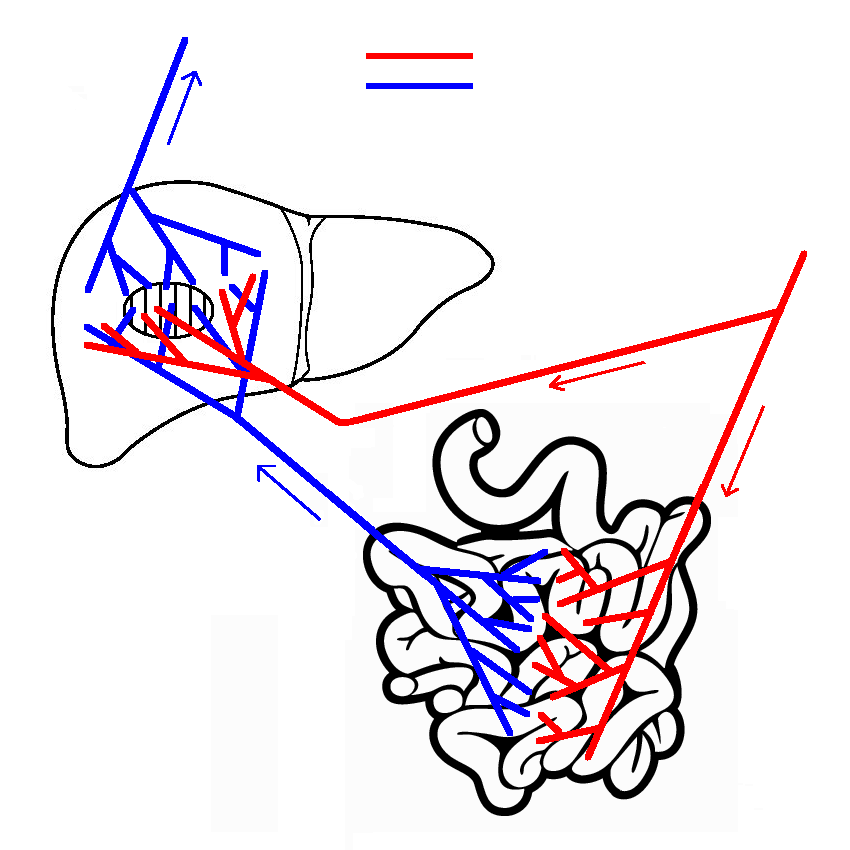
\includegraphics[width=100\unitlength]{schema/schema_irrigation_foie.png}}

%%% Cadre bordure
%\put(0,0){\line(0,1){100}}\put(0,0){\line(1,0){100}}
%\put(100,0){\line(0,1){100}}\put(0,100){\line(1,0){100}}

\put(57,92.5){Sang artériel, riche en oxygène}
\put(57,89){Sang veinal, pauvre en oxygène}

\put(40,75){Foie}
\put(82,18){Intestin grêle}
\put(82,15){et autres}
\put(83,12){organes du}
\put(82,9){tube digestif }

\linethickness{0.4\unitlength}
\put(18,65){\line(-10,-30){10}}
\put(1,32){Métastase}
\put(1,29){hépatique}

\put(57,56){ \begin{turn}{15} Artère hépatique \end{turn} }
\put(11,78){ \begin{turn}{70} Veine hépatique \end{turn} }
\put(31,49){ \begin{turn}{-40} Veine porte \end{turn} }
\put(77.5,48){ \begin{turn}{66} Artère \end{turn} }
\put(79,44){ \begin{turn}{66} mésentérique \end{turn} }
\end{picture}
